% !TeX program = xelatex
\documentclass[3pt,landscape]{article}
\usepackage{multicol, calc, ifthen, amsmath, amsthm, amsfonts, amssymb, color, graphicx, overpic, hyperref, fontspec, xunicode}

\usepackage[landscape]{geometry}

\defaultfontfeatures{Mapping=tex-text,Scale=MatchLowercase}
\ifthenelse{\lengthtest { \paperwidth = 11in}}
    { \geometry{top=.3in,left=.3in,right=.3in,bottom=.3in} }
    {\ifthenelse{ \lengthtest{ \paperwidth = 297mm}}
        {\geometry{top=1cm,left=1cm,right=1cm,bottom=1cm} }
        {\geometry{top=1cm,left=1cm,right=1cm,bottom=1cm} }
    }
\pagestyle{empty}
\makeatletter
\setmainfont{Source Sans Pro}
\setmonofont{Menlo}
\DeclareMathSizes{3}{3}{2}{1}

\renewcommand{\section}{\@startsection{section}{1}{0mm}{-1ex plus -.5ex minus -.2ex}{0.5ex plus .2ex}{\normalfont\large\bfseries}}
\renewcommand{\subsection}{\@startsection{subsection}{2}{0mm}{-1explus -.5ex minus -.2ex}{0.5ex plus .2ex}{\normalfont\normalsize\bfseries}}
\renewcommand{\subsubsection}{\@startsection{subsubsection}{3}{0mm}{-1ex plus -.5ex minus -.2ex}{1ex plus .2ex}{\normalfont\small\bfseries}}
\makeatother
\setcounter{secnumdepth}{0}
\setlength{\parindent}{0pt}
\setlength{\parskip}{0pt plus 0.5ex}
\hypersetup{colorlinks=true, urlcolor=blue}
\def\ci{\perp\!\!\!\perp}

%%%%%%%%%%%%%%%%%%%%%%%%%%%%%%%%%%%%%%%%%%%%%%%%%%

\begin{document}
\raggedright
\footnotesize

\begin{multicols}{3}
\setlength{\premulticols}{1pt}
\setlength{\postmulticols}{1pt}
\setlength{\multicolsep}{1pt}
\setlength{\columnsep}{2pt}

\begin{center}
    \Large{\underline{Algorithms Mini Field Guide 1.0}} \\
\end{center}
\begin{center}
    Written by: \href{http://krishna.im}{Krishna Parashar}\\
    Published by: \href{http://www.ocm.io}{The OCM}\\
\end{center}

%%%%%%%%%%%%%%%%%%%%%%%%%

\subsection*{Basic Properties of Logarithms}
$y = \log _b \left( x \right){\rm{ iff }}x = b^y$\\
$\log _b \left( {xy} \right) = \log _b \left( x \right) + \log _b \left( y \right)$\\
$\log _b \left( x \right) = \log _b \left( c \right)\log _c \left( x \right) = \frac{{\log _c \left( x \right)}}{{\log _c \left( b \right)}}$\\
$\log _b \left( {x^n } \right) = n\log _b \left( x \right)$
$x^a x^b  = x^{\left( {a + b} \right)}$
$\left( {x^a } \right)^b  = x^{\left( {ab} \right)}$
$x^{\left( {\frac{1}{2}} \right)}  = \sqrt x$
$x^{\left( {a - b} \right)}  = \frac{{x^a }}{{x^b }}$

\subsection*{Basic Series}
Arithmetic Series (Sequential Integers): $\sum\limits_{k = 1}^n {k = \frac{{n\left( {n + 1} \right)}}{2}}$\\
Arithmetic Series (Sequential Odd Ints): $\sum\limits_{k = 1}^n {2k - 1 = n^2 }$\\
Artihmetic Series (Square): $\sum\limits_{k = 1}^n {k^2  = \frac{{n\left( {n + 1} \right)\left( {2n + 1} \right)}}{6}}$
Finite Geometric Series: $\sum\limits_{k = 1}^n {ar^{k - 1}  = \frac{{a\left( {1 - r^n } \right)}}{{1 - r}}}$ \\
Infinite Geometric Series: $\sum\limits_{k = 1}^\infty  {ar^{k - 1}  = \frac{a}{{1 - r}}}$

\subsection*{Formal Limit Definition of \(O, \Theta, \texttt{and } \Omega\)}
\[\lim_{n \rightarrow \infty}\frac{f(n)}{g(n)}\left\{\begin{array}{lr}
            \geq 0(\infty) & f(n) \in \Omega(g(n))\\
            < \infty(0) & f(n) \in O(g(n))\\
            = c, 0 < c < \infty & f(n) \in \Theta(g(n))
    \end{array}\right.\]

\subsection*{Topological Sort $O(V + E)$}

Constraints: A directed graph G is acyclic if and only if a depth-first search of G yields no back edges. Formally, we say a topological sort of a directed acyclic graph G is an ordering of the vertices of G such that for every edge $(v_i, v_j)$ of G we have $i < j$. If DAG is cyclic then no linear ordering is possible.

\textbf{Topological Sort} returns a list with all nodes pointing left such that basically all parents come before any children (excluding sources).
We order a graph from the \textbf{highest post number} in a decreasing order. \\

Thus we create singly connected component from a DAG with several strongly connected components, each a unique source and unique sink in the DAG. There are multiple topological sorting possible. Used for Runtime Compiling or Scheduling.

\begingroup
    \fontsize{6pt}{6pt}\selectfont
\begin{verbatim}
pre/post 
[u[v v]u] is a Tree/Forward Edge
[v[u u]v] is a Back Edge
[v v][u u] is a Cross Edge
\end{verbatim}
\endgroup

\subsection*{Master's Theorem}
If
\[T(n)=aT(\lceil n/b \rceil)+O(n^{d}) \texttt{ for } a>0,b>1 \texttt{, and } d\geq 0,\]
then,
\[T(n)=\left\{\begin{array}{lr}
            O(n^{d}) & if d>log_{b}a\\
            O(n^{d}logn) & if d=log_{b}a\\
            O(n^{log_{b}a}) & if d < lob_{b}a\\
        \end{array}
        \right.\]
    Branching Factor: $a$\\
    Depth of Tree = $log_{b}n$\\ 
    Width of Tree: $a^{log_{b}n} = n^{log_{b}a}$

\iffalse
\subsection*{Volker Strassen}
Divide and conquer matrix multiplication.\\
Matrix multiplication can be broken into subproblems, because it can be performed blockwise. Ex, we can carve X into for \(n/2\) x \(n/2\) blocks
\[X = \begin{bmatrix} A & B \\ C & D \end{bmatrix}, Y = \begin{bmatrix} E & F\\ G & H \end{bmatrix}\]
Then the product can be expressed in terms of those blocks as if the blocks were a single element,
\[XY = \begin{bmatrix} A & B \\ C & D \end{bmatrix} * \begin{bmatrix} E & F\\ G & H \end{bmatrix} = \begin{bmatrix} AE+BG & AF+BH \\ CE+DG & CF+DH \end{bmatrix}\]
The runtime of this recurrence is,
\[T(n)=8T(n/2)+O(n^{2}) \rightarrow O(n^{3})\]
Using clever algebra, this can be improved with integer multiplication, XY can be computed from seven \(n/2\) x \(n/2\) subproblems via decomposition.
\[XY = \begin{bmatrix} P_{5}+P_{4}-P_{2}+P_{6} & P_{1}+P_{2} \\ P_{3}+P_{4} & P_{1}+P_{5}-P_{3}+P_{7} \end{bmatrix}\]
where,
\[\begin{array}{ll}
        P_{1}=A(F-H) & P_{2}=(A+B)H\\
        P_{3}=(C+D)E & P_{4}=D(G-E)\\
        P_{5}=(A+D)(E+H) & P_{6}(B-D)(G+H)\\
        P_{7}=(A-C)(E+F) & \texttt{ }
\end{array}\]
and has a runtime of
\[T(n)=7T(n/2)+O(n^{2}) \rightarrow O(n^{log_{2}7}) \approx O(n^{2})\]
\fi

\subsection*{Fast Fourier Transform \(O(n\log{n})\)}
The Fast Fourier Transform in the scope of our knowledge thus far is used for Polynomial Multiplication. We want to know the coefficient of $(p \cdot q)(x)$ knowing only the coefficients of $p(x)$ and $q(x)$. The naive way is the one we all use in Algebra which runs in \(O(n^2)\). Here is a faster algorithm:

\begin{enumerate}
  \item Take the coefficients of $p(x)$ and $q(x)$ and plug them into the FFT with the Roots of Unity (We need $2n+1$ points). \(O(n\log{n})\)
  \item From the FFT we get the roots of unity evaluated at $p(x)$ and $q(x)$ and we multiply the respected values from each root together to get $2n+1$ respective pairs of values of $(p \cdot q)(x)$. \(O(n)\)
  \item Finally we interpolate these points using the inverse FFT to get the coefficients of $(p \cdot q)(x)$. \(O(n\log{n})\)
\end{enumerate}
\textbf{Evaluation: }$<values>$ = FFT($<coeff>$, $w$)\\
\textbf{Interpolation: }$<coeff>$ = ($1/n$) FFT($<values>$, $w^{-1}$)\\

\begin{verbatim}
function FFT(A, w)
Input: Coefficient representation of a polynomial A(x)
of degree less than or equal to n−1, 
where n is a power of 2w, an nth root of unity
Output: Value representation A(w_0),...,A(w_n−1)

if w = 1: return A(1)
express A(x) in the form A_e(x^2) + xA_o(x^2)
call FFT(A_e, w^2) to evaluate A_e at even powers of w 
call FFT(A_o, w^2) to evaluate A_o at even powers of w 
for j = 0 to n − 1:
   compute A(w_j) = A_e(w^2j) + w^j A_o(w^2j) 
return A(w_0),...,A(w_n−1)
\end{verbatim}

\iffalse
\textbf{Roots of Unity: }\\
complex \(n^{th}\) roots of unity are given by \(e^{\frac{2 \pi i}{n}}\)
The Vandermonde Matrix,
\[M_{n}(\omega) =
    \begin{bmatrix}
        1 & 1 & 1 & \cdots & 1\\
        1 & \omega & \omega^{2} & \cdots & \omega^{n-1}\\
        1 & \omega^{2} & \omega^{4} & \cdots & \omega^{2(n-1)}\\
        \vdots & \vdots & \vdots & \ddots & \vdots\\
        1 & \omega^{j} & \omega^{2j} & \cdots & \omega^{(n-1)j}\\
        \vdots & \vdots & \vdots & \ddots & \vdots\\
        1 & \omega^{(n-1)} & \omega^{2(n-1)} & \cdots & \omega^{(n-1)(n-1)}
\end{bmatrix}\]
\fi
This process happens recursively. 

\subsection*{Search Algorithms}

\subsubsection*{Depth First Search \(O(V + E)\) (Stack)}
Explores all the way down to a tree, then climbs back up and explores alt paths. Use for Topological Sort and Finding Connected Components.
$(pre(u) < pre(v) < post(v) < post(u))$\\

\begin{verbatim}
def explore(G,v): #Where G = (V,E) of a Graph
Input: G = (V,E) is a graph; v ∈ V
Output: visited(u) is set to true for all nodes u 
reachable from v
    visited(v) = true
    previsit(v)
    for each edge(v,u) in E:
        if not visited(u):
            explore(u)
    postvisit(v)

def dfs(G):
    for all v in V:
        if not visited(v):
            explore(v)
\end{verbatim}
\textbf{Previsit} = count till node added to the queue\\
\textbf{Postvisit} = count till you leave the given node\\
A directed Graph has a cycle if and only if it a back edge found during DFS.

\subsubsection*{Strongly Connected Components $O(n)$}
Us for most edge removal problems, use this to check if still strongly connected.\\
\textbf{Properties: }
\begin{itemize}
\item If the explore subroutine is started at node u, then it will terminate precisely when all nodes reachable from u have been visited.
\item The node that receives the highest post number in a depth-first search must lie in a source strongly connected component.
\item If C and C′ are strongly connected components, and there is an edge from a node in C to a node in C′, then the highest post number in C is bigger than the highest post number in C′.
\end{itemize}
\textbf{Run Time: }$O(n)$\\
\textbf{Big Picture: }Topologically sort the graph; reverse the edges; topologically sort again; ff we reach a new source the resulting traversal is new SCC; continue till end of list. \\

Algorithm:
\begin{itemize}
\item  Run depth-first search on G.\\
\item Run the undirected connected components algorithm (which count uses a counter to count the number of components in G) on G, and during the depth-first search, process the vertices in decreasing order of their post numbers from step 1.
\end{itemize}


\subsubsection*{Breadth First Search \(O(V + E)\) (Queue)}
\begin{verbatim}
Input: Graph G = (V, E), directed or undirected; vertex s ∈ V 
Output: For all vertices u reachable from s, dist(u) is set
to the distance from s to u.

def bfs(G,s):
    for all u in V:
        dist(u) = infinity
    dist(s) = 0
    Q = [s] (Queue containing just s)
    while Q is not empty:
        u = eject(u)
        for all edges (u,v) in E:
            if dist(v) = infinity:
                inject(Q,v)
                dist(v) = dist(u) + 1
\end{verbatim}


\subsubsection*{Dijkstra's Algorithm $O(V + E)\log{V}$ (Binary Heap)}
Objective is to find shortest path.
Standard Data Structure is Priority Queue.
\begin{verbatim}
def dijkstra(G,l,s):
    for all u in V:
        dist(u) = infinity
        prev(u) = nil
    dist(s) = 0
    H = makequeue(V) # using dist values as keys
    while H is not empty:
        u = deletemin(H)
        for all edges (u,v) in E:
            if dist(v) > dist(u)+l(u,v)
                dist(v) = dist(u)+l(u,v)
                prev(v) = u
                decreasekey(H,v)
\end{verbatim}

\subsubsection*{Bellman Ford Algorithm $O(V \cdot E)$}
Objective is to find shortest path allowing for \textbf{negative edges}. 
\begin{verbatim}
procedure shortest-paths(G, l, s)
Input: Directed graph G = (V, E); 
edge lengths {l_e: e in E} with no negative cycles; 
vertex s in V
Output: For all vertices u reachable from s, 
dist(u) is set to the distance from s to u.
for all u in V: 
    dist(u) = infinity 
    prev(u) = nil

dist(s) = 0
repeat |V|-1 times:
    for all e in E: 
        update(e)
\end{verbatim}

\subsection*{Directed Acyclic Graphs}
\begin{itemize}
    \item Every DAG has a source and sink
    \item A directed graph has a cycle if and only if its depth-first search reveals a back edge.
    \item In a DAG, every edge leads to a vertex with a lower post number.
    \item Every directed graph is a DAG of its strongly connected components.
    \item If the explore subroutine is started at node u, then it will terminate precisely when all nodes reachable from u have been visited
    \item The node that receives the highest post number in a depth-first search must lie in a source strongly connected component
    \item If C and C' are strongly connected components, and there is an edge from a node in C to a node in C', the the highest post number in C is bigger than the highest post number in C'.
    \item In any path of a DAG, the vertices appear in an increasing linearized order allowing you to run Dijkstra's Algorithm in \(O(n)\)
\end{itemize}

\subsection*{Greedy Algorithms}

\subsubsection*{Definitions}
A \textbf{Greedy Algorithm} always takes the cheapest least weight edge for its next step, no matter the future consequences.\\
A \textbf{Tree} is an acyclic, undirected, connected graph with $|V| - 1$ edges (or for \textit{MST} exactly $|V| - 1$ edges).\\
A \textbf{Fringe} is all the vertices exactly one hop from you current vertex.\\

\subsubsection*{Kruskal's MST Algorithm \(O(E\log{E})\)}
\textbf{(If Dense: $|E|$ at most $|V^2|$)}\\
Sort edges using a sorting algorithm then repeatedly add the next lightest edge that doesn't produce a cycle (i.e. only visit new vertices).
\begin{verbatim}
Input: A connected undirected graph G = (V,E) with edge 
        weights w
Output: A minimum spanning tree defined by the edges X

for all u in V:
    makeset(u)
X = {}
Sort the edges E by weight
for all edges {u,v} in E, in increasing order of weight:
    if find(u) != find(v):
        add edge {u,v} to X
        union(u,v)
\end{verbatim}
The above algorithm utilizes disjoint sets to determine whether adding a given edge creates a cycle. Basically by checking whether or not both sets have the same root ancestor.
\begin{center}
    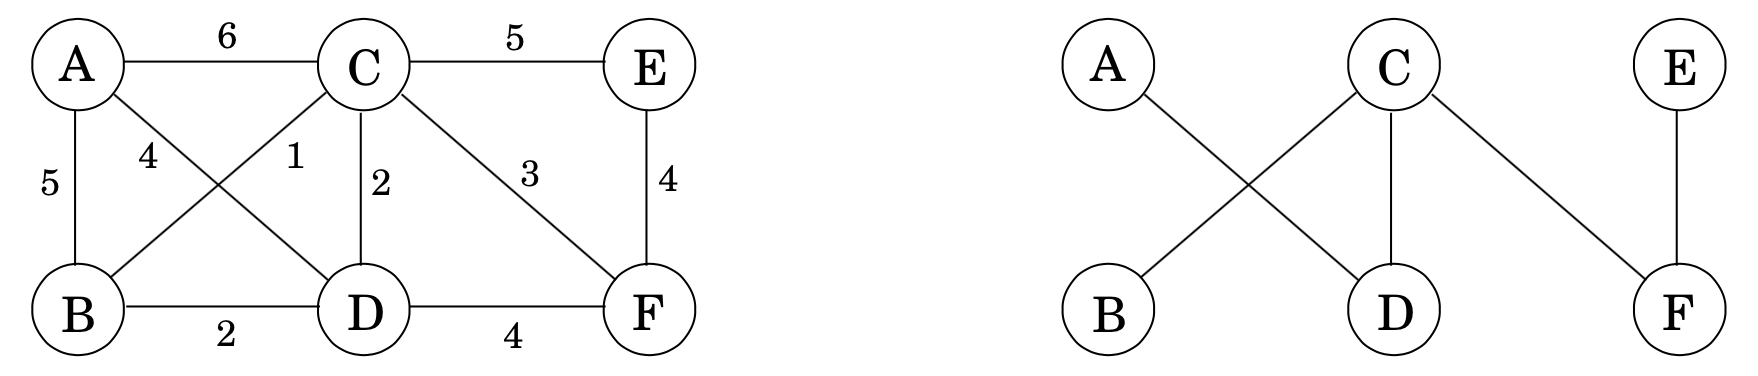
\includegraphics[height=1cm]{kruskal-example.png}
\end{center}

\subsubsection*{Properties of Trees (Undirected Acyclic Graphs)}
\begin{itemize}
    \item A tree with n nodes has n-1 edges
    \item Any connected undirected graph G(V,E), with \(|E|=|V|-1\) is a tree
    \item An undirected graph is a tree if and only if there is a unique path between any pair of nodes.
\end{itemize}

\subsubsection*{Cut Property}
Suppose edges X are part of a minimum spanning tree of \(G=(V,E)\). Pick any subset of nodes S for which X does not cross between S and V-S, and let e be the lightest edge across the partition. Then \(X \cup {e}\) is part of some Minimum Spanning Tree.

\subsubsection*{Prim's Algorithm \(O(E\log{E})\)}
Objective is to also find the MST.
Alternative to Kruskal's Algorithm; Similar to Dijkstra's)\\
Standard Data Structure is Priority Queue.
\textbf{(If Dense: $|E|$ at most $|V^2|$)}\\
On each iteration, the subtree defined by x grows by one edge, the lightest between a vertex in S and a vertex outside S.

\begin{verbatim}
procedure prim(G, w)
Input: A connected undirected graph G = (V, E) with weights
Output: A minimum spanning tree defined by the array prev
for all u in V : 
    cost(u) = infinity
    prev(u) = nil
Pick any initial node u_0 
cost(u_0) = 0
H = makequeue (V) (priority queue with cost-values as keys) 
while H is not empty:
    v = deletemin(H) 
        for each {v, z} in E:
            if cost(z) > w(v, z): 
                cost(z) = w(v, z) 
                prev(z) = v 
                decreasekey(H, z)
\end{verbatim}
\begin{center}
    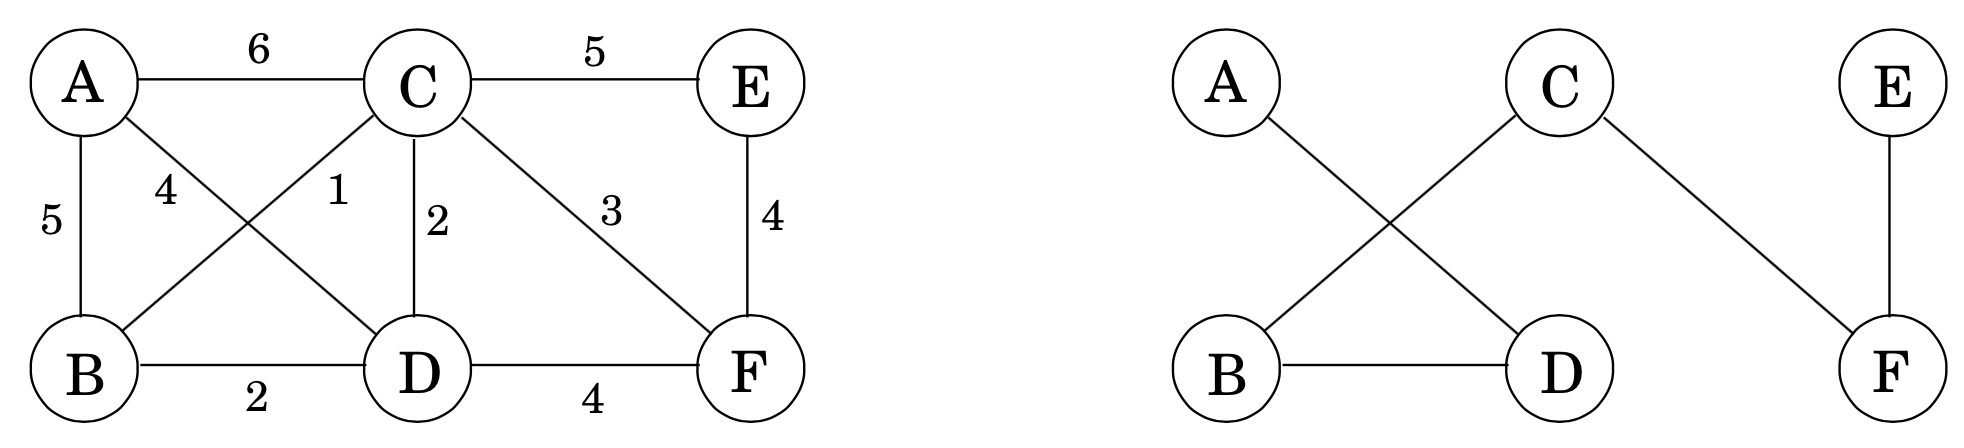
\includegraphics[height=1cm]{prims-example.png}
\end{center}

\subsubsection*{Huffman Encoding}
A means to encode data using the optimal number of bits for each character given a distribution.

\subsubsection*{Set Cover Algorithm (Polynomial Time)}
\begin{verbatim}
Input: A set of elements B; sets S1,...,Sm
Output: A selection of the S_i whose union is B.
Cost: Number of sets picked.

Repeat until all elements of B are covered:
    Pick the set Si with the largest number of
            uncovered elements.
\end{verbatim}

\subsubsection*{Disjoint Sets Data Structure}
Contains a function, "find" that returns the root a given set.
$pi$ refers to the parent node.
$rank$ refers to the height subtree hanging form that node (number of levels below it).
\begin{itemize}
\item For any $x, rank(x) < rank(\pi(x))$.
\item Any root node of rank $k$ has at least $2^k$ nodes in its tree.
\item If there are $n$ elements overall, there can be at most $\frac{n}{2^k}$ nodes of rank $k$. The maximum rank is $log n$.
\end{itemize}
\begin{verbatim}
def makeset(x): // O(1)
    pi(x) = x
    rank(x) = 0

def find(x): // O(E log V)
    while x != pi(x):
        x=pi(x)
    return x

def union(x,y): // O(E log V)
    if find(x) == find(y):
        return
    elif rank(find(x)) > rank(find(y)):
        pi(find(y)) = find(x)
    else:
        pi(find(x))=find(y)
        if rank(find(x)) == rank(find(y)):
            rank(find(y)) = rank(find(y)) + 1
\end{verbatim}

\subsubsection*{Path Compression}
\begin{verbatim}
function find(x): 
    if x != pi(x): pi(x) = find(pi(x)) 
    return pi(x)
\end{verbatim}
Using path compression allows for an amortized cost of O(1) for out Disjoint Set's $union(x, y)$ and $find(x)$ operations.

\subsubsection*{Union Find}
Uses Disjoint Sets Data Structure\\
Runs in per operation $Olog*{n}$ which is the number of times you can take a log of n before it becomes 1 or less. It is very slow and for all practical cases is constant. \\
Basically if find(x) and find(y) return the same value they are in the same graph so do nothing, else add the edge. Then union(x, y).

Union: Worst case is $O(logN)$ Avg for all Ops is $O(nlog*{n})$ where n is number of elements in Data Structure.

% You can even have references
\rule{0.3\linewidth}{0.1pt}
\scriptsize
\bibliographystyle{abstract}
\bibliography{refFile}
\end{multicols}
\end{document}
